\section{Levels of recursion and limits on human reasoning}
\label{sec:levels}

In our next set of experiments, \exptrefrange{exp:levels-levels}{exp:levels-size}, we probed limits on the kind of inferences we could measure in our reference game paradigm. In all of these experiments, we also conducted parallel experiments measuring prior expectations using the methods described in \secref{sec:priors}, but we largely omit discussion of these data until \secref{sec:models}.

In our first experiment, \exptref{exp:levels-level}, we attempted to measure patterns of inference in more complex reference games. Following \citeA{stiller2011} and \citeA{degen2012}, we created a matrix that required a deeper level of reasoning than our previous experiments. In particular, we compared our standard reference game (shown again for reference in Figure \ref{fig:levels-level}A) with a more complex game (Figure \ref{fig:levels-level}B). In the standard game, we measured the level at which participants chose the pragmatic target, which we call a Level 1 inference (we return to this notation in \secref{sec:models}). We also measured the level of choosing the target with the unique feature (e.g. choosing the hat with the word ``hat''; a ``level 0'' inference). In the more complex game, we measured the standard Level 1 inference (the target for this inference was the face with a mustache but no glasses, for the utterance ``mustache''). The contribution of this experiment, however, was our test of a Level 2 inference (``glasses,'' with the presumptive target the face with glasses and mustache, not glasses and hat). This inference depends on having reasoned that while both of the targets have another possible descriptor, for one of those targets, the second descriptor is unique, whereas for the other the second descriptor is also non-unique. 




 \begin{figure}[t]
  \centering
  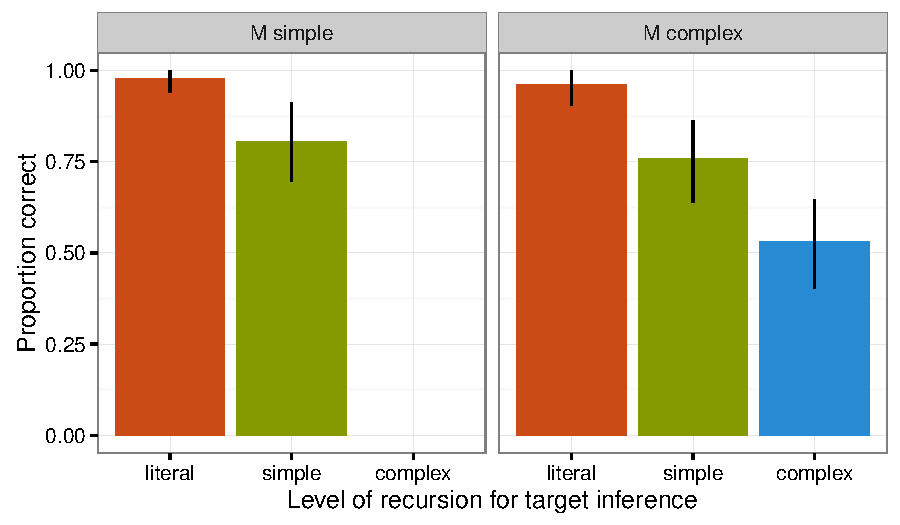
\includegraphics[width=4in]{../plots/3-levels-levels.pdf}\\ 
  A) 
\includegraphics[width=3in]{figures/hatglasses.pdf}\\
  B) 
\includegraphics[width=3in]{figures/levels-levels-stim.pdf}
  \caption{\label{fig:levels-level} Data from \exptref{exp:levels-level} in the inference conditions.}
\end{figure}


 \begin{figure}[t]
  \centering
  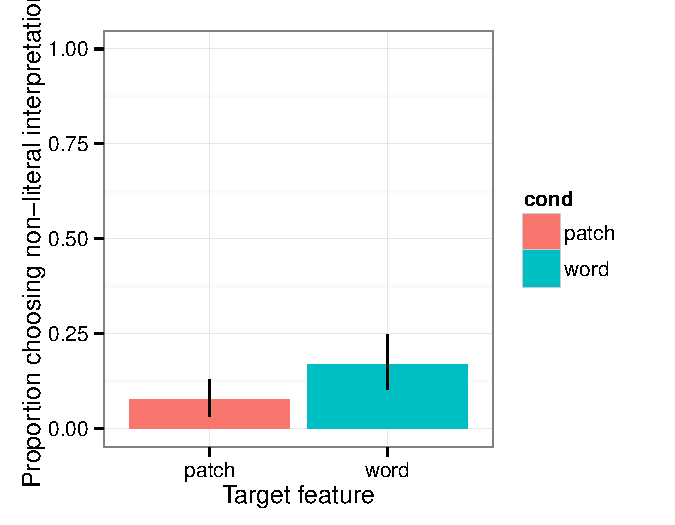
\includegraphics[width=4in]{../plots/3-levels-oddman.pdf}
  
\includegraphics[width=4in]{figures/levels-oddman-stim.pdf}
  \caption{\label{fig:levels-levels} Data from \exptref{exp:levels-oddman} in the inference conditions.}
\end{figure}

 \begin{figure}[t]
  \centering
  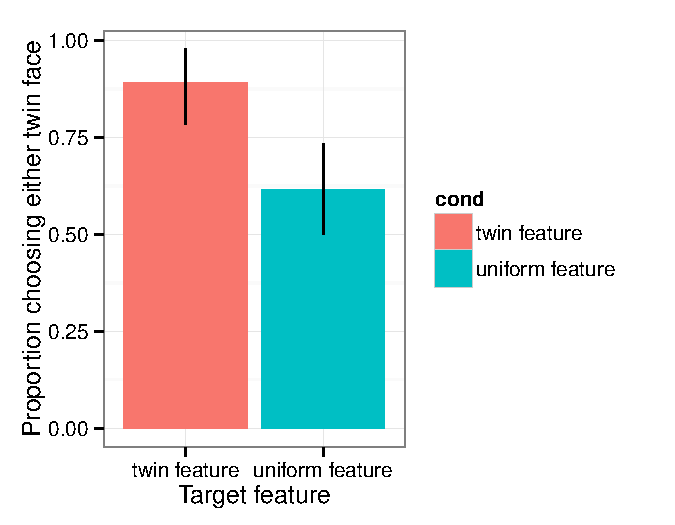
\includegraphics[width=4in]{../plots/3-levels-twins.pdf}
  
\includegraphics[width=4in]{figures/levels-twins-stim.pdf}
  \caption{\label{fig:levels-levels} Data from \exptref{exp:levels-twins} in the inference conditions.}
\end{figure}

 \begin{figure}[t]
  \centering
  % \includegraphics[width=4in]{../figures/3-levels-size-stim.pdf}
  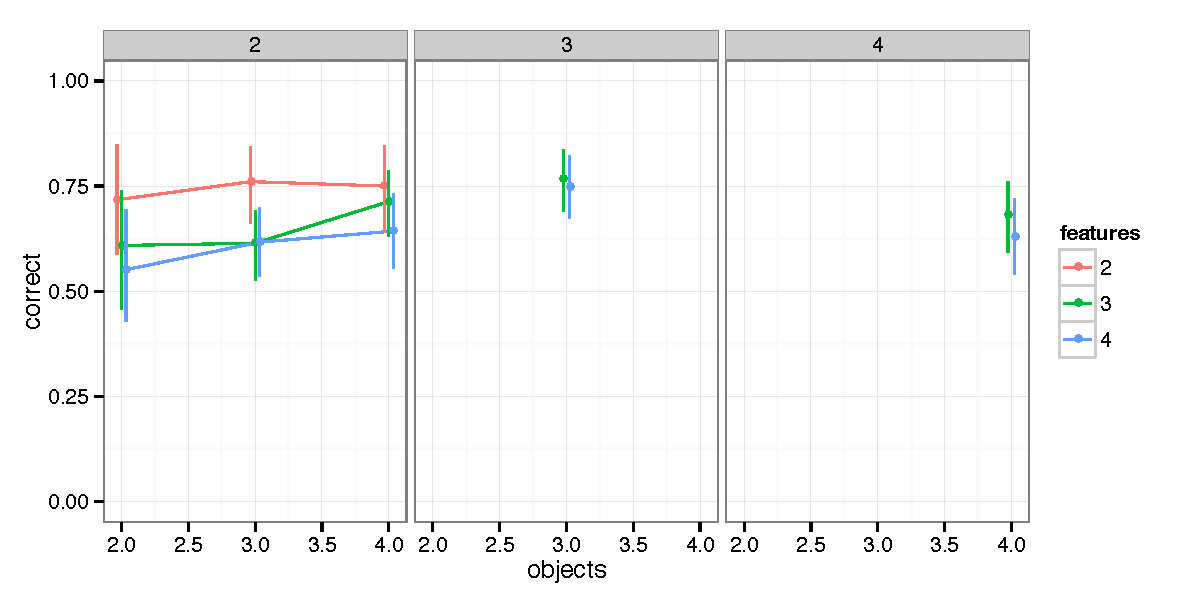
\includegraphics[width=4in]{../plots/3-levels-size.pdf}
  \caption{\label{fig:levels-levels} Data from \exptref{exp:levels-size} in the inference conditions.}
\end{figure}